\documentclass[12pt,a4paper]{article}
\usepackage{pgf}
% \usepackage[condensed,math]{kurier}
% \usepackage[T1]{fontenc}
\usepackage{svg}
\usepackage{tikz}
\usepackage{stanli}
\usepackage{afterpage}
\usepackage{multirow}
\usepackage{subfig}
\usepackage{pgfpages}
\usepackage{listings}
\usepackage{rotating}

\usepackage{xcolor}

\definecolor{codegreen}{rgb}{0,0.6,0}
\definecolor{codegray}{rgb}{0.5,0.5,0.5}
\definecolor{codepurple}{rgb}{0.58,0,0.82}
\definecolor{backcolour}{rgb}{0.95,0.95,0.92}

\lstdefinestyle{mystyle}{
    backgroundcolor=\color{backcolour},   
    commentstyle=\color{codegreen},
    keywordstyle=\color{magenta},
    numberstyle=\tiny\color{codegray},
    stringstyle=\color{codepurple},
    basicstyle=\ttfamily\footnotesize,
    breakatwhitespace=false,         
    breaklines=true,                 
    captionpos=b,                    
    keepspaces=true,                 
    numbers=left,                    
    numbersep=5pt,                  
    showspaces=false,                
    showstringspaces=false,
    showtabs=false,                  
    tabsize=2
}

\lstset{style=mystyle}

%\usepackage{times}


\pgfpagesdeclarelayout{boxed}
{
	\edef\pgfpageoptionborder{0pt}
}
{
	\pgfpagesphysicalpageoptions
	{%
		logical pages=1,%
	}
	\pgfpageslogicalpageoptions{1}
	{
		border code=\pgfsetlinewidth{2pt}\pgfstroke,%
		border shrink=\pgfpageoptionborder,%
		resized width=.9\pgfphysicalwidth,%
		resized height=.9\pgfphysicalheight,%
		center=\pgfpoint{.5\pgfphysicalwidth}{.5\pgfphysicalheight}%
	}%
}

\pgfpagesuselayout{boxed}


% Language setting
% Replace `english' with e.g. `spanish' to change the document language
\usepackage[english]{babel}
\usepackage{csvsimple}
% Set page size and margins
% Replace `letterpaper' with `a4paper' for UK/EU standard size
\usepackage[a4paper,top=2cm,bottom=1.5cm,left=1.5cm,right=1.5cm]{geometry}

% Useful packages
\usepackage{amsmath}
\usepackage{graphicx}
\usepackage[colorlinks=true, allcolors=blue]{hyperref}

\title{}
\author{}
\date{}

\begin{document}

\newcommand{\subf}[2]{%
    {\small\begin{tabular}[t]{@{}c@{}}
                #1 \\#2
            \end{tabular}}%
}

\begin{titlepage}
    \begin{center}
        \vspace*{3cm}

        \Huge
        \textbf{Simulation and Models: Report}

        \vspace{0.3cm}
        \Huge
        Project 1

        \vspace{0.8cm}
        \large

        %INSTRUCTED BY: MRS. A.A.S.KAUSHLYA


        \vspace{0.5cm}
        \LARGE


        \vspace{1.5cm}

        \textbf{}
        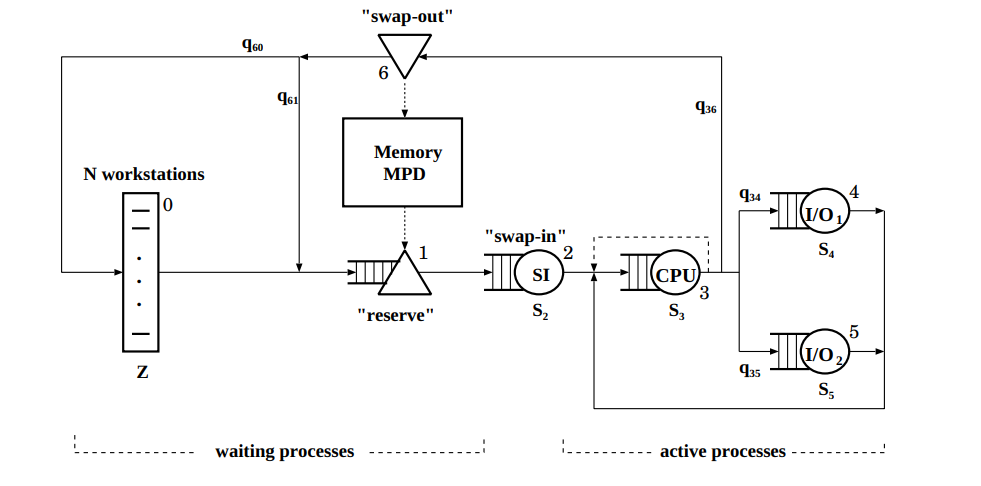
\includegraphics[width=0.8\textwidth]{./Images/model.png}

        \vfill



        \vspace{0.8cm}



        \Large




    \end{center}
    \Large
    \begin{tabbing}
        \hspace*{1em}\= \hspace*{8em} \= \kill % set the tabbings
        \> Name:\>  \textbf{Matteo Ielacqua} \\
        \> ID:\>  \textbf{839241} \\
    \end{tabbing}

\end{titlepage}



\section{Description of the simulator}
In this section a brief analysis of the code and other technical aspect of the simulator will be discussed.
\subsection{Events}
The simulator is designed to manage a range of events within this system, with a particular focus on two crucial types: the arrival of a client and the departure. Each event type has a distinct impact on the simulator's state, influenced by the specific target under consideration.
\subsubsection{Delay station}

\textbf{Departure from the delay station}: The client leaving the delay station will be scheduled for arrival to the Reserve station.
\\
\textbf{Arrival at the delay station}:
an arrival will trigger a departure with a certain delay, that is a Random Variable with a negative exponential distribution with expected value of 5000 ms
\\
\subsubsection{Reserve station}
\textbf{Arrival at the Reserve station:} if the counter of the process allocated in the system is less than the MPD. Then the  arrival event is immediately scheduled for the swap in. Otherwise, the information are stored in a queue and used when a process will exit from the swap out (and the counter decremented).

\subsubsection{Swap in}
\textbf{Arrival at the swap in station:} when a client arrive 2 behavior can happen: 1) the client arrives and found the queue empty, then it will be immediately scheduled for departure with a delay based on an exponential RV with expected value of 210 ms. 2) the client find the station busy, then it will be enqueued for later processing with FCFS policy.
\\
\textbf{Departure from the swap in station:} a departure from the swap in will trigger an immediate arrival at the CPU.


\subsubsection{CPU}
\textbf{Arrival at the CPU}: when a process arrives at the CPU a service time based on a hyper exponential distribution is assigned and then 2 things can happen. 1) The CPU is not busy, then the current process will occupy the CPU and a departure will be scheduled for a time equivalent to the actual clock plus time slice, the same time will be decreased from the remaining service time of the process. 2) The CPU is busy, then the process will be enqueued in the process queue.
\\
\textbf{Departure from the CPU}: A process can leave the CPU only when its service time is 0. So when a departure is scheduled 2 case exists: 1) The process's service time is > 0, in this case the process is enqueued again in the process queue. 2) The process's service time is 0, in this case the next station will be randomly chosen (using proper probabilities) and the event will be scheduled as arrival for that station. If there is a process in the queue, after those operations, it will be dequeued and processed by the CPU using the same mechanism described for the arrivals.

\subsubsection{IO}

\textbf{Arrival to IO1/IO2:} in both cases an arrival will trigger a departure from the relative station that is an RV with negative exponential distribution.
\\
\textbf{Departure from IO1/IO2:} in both cases this will result in an immediate arrival event to the CPU.

\subsubsection{Swap Out}
\textbf{Arrival to swap out:} this event will trigger an immediate departure for the swap out
\\
\textbf{Departure from swap out:} this event will trigger an immediate arrival to the delay station with p 0.4 or an immediate arrival to the reserve station with p 0.6. In any case this event will decrement by 1 the counter of allocated process in the reserve station.


\subsection{Choice of the regeneration point}
The regeneration point is chosen starting from some pilot simulation. In those simulations when the tagged customer exit the swap out the current status of the simulator is collected. After 1000 runs those where most recognized observed state when this kind of event happen.
\begin{verbatim}
    NDelay:3, NReserve:7, NSwap:0, NCPU:0, NIO1:0, NIO2:9,NOUT:0, hits:18
    NDelay:5, NReserve:5, NSwap:0, NCPU:0, NIO1:0, NIO2:9,NOUT:0, hits:16
    NDelay:3, NReserve:7, NSwap:0, NCPU:0, NIO1:1, NIO2:8,NOUT:0, hits:16
    NDelay:2, NReserve:8, NSwap:0, NCPU:0, NIO1:0, NIO2:9,NOUT:0, hits:15
\end{verbatim}
The sum of clients in this print-out is always 19 because the measure is taken when the client is exiting the swap out, so the tagged customer is not counted. In this case a good fit is 0 clients at the CPU , 0 clients at the IO1 and 9 at the IO2, 3 at the delay station and 7 at the Reserve. The regeneration point will be then evaluated each time the tagged customer approach the swap out and if the conditions are met then the measure will be collected and the accumulators reset.

\section{Simulation results}
The following subsection will illustrate 4 different scenarios of execution:
\begin{enumerate}
    \item Default scenario: the CPU has a Hyper exponential distribution of service time and a fixed slice time of 2.7 ms.
    \item NegExp scenario: the CPU has a negative exponential distribution of service time and a fixed time slice of 2.7 ms.
    \item LTCpu: the CPU has a hyper exponential distribution of service time and a fixed time slice of 2700 ms.
    \item NegExpLT: the CPU has a negative exponential distribution of service time and a fixed time slice of 2700 ms.
\end{enumerate}
Legend for Plots:
\begin{itemize}
    \item LB = Lower Bound of interval 
    \item HB = Higher bound of interval 
    \item R = point estimator
\end{itemize}

\subsection{Default scenario}
In the default scenario despite having 20 clients the active part of the system has never more then 10 clients.
\includegraphics[width=0.9\textwidth]{./Images/meanActiveTime_Default.png}

\includegraphics[width=0.9\textwidth]{./Images/Default_CPU_meanclients.png}

\includegraphics[width=0.9\textwidth]{./Images/Default_CPU_meanwaits.png}

this is possible because the Reserve Station is limiting the number of clients that can be present in the active part of the system. Thus reducing the size of the queues in the system. If this station is not present, then probably the system would experience trashing, due to the high service time of IO2.

\begin{table}[!ht]
    \centering
    \begin{tabular}{|l|l|l|l|l|l|l|l|}
    \hline
        Station & Measure & R & LB & HB & Samples & Precision & Expected \\ \hline
        CPU & meanclients & 1.37289 & 1.33024 & 1.41554 & 154 & 0.03107 & 1.47487 \\ \hline
        CPU & meanwaits & 5.97389 & 5.84747 & 6.1003 & 154 & 0.02116 & 6.65303 \\ \hline
        IO1 & meanclients & 1.28732 & 1.26081 & 1.31382 & 154 & 0.02059 & 1.34865 \\ \hline
        IO1 & meanwaits & 89.46688 & 88.13577 & 90.79798 & 154 & 0.01488 & 93.59424 \\ \hline
        IO2 & meanclients & 6.44702 & 6.37445 & 6.51959 & 154 & 0.01126 & 11.87475 \\ \hline
        IO2 & meanwaits & 1171.2056 & 1155.19151 & 1187.21969 & 154 & 0.01367 & 2142.63856 \\ \hline
        SWAP\_IN & meanclients & 0.86811 & 0.83884 & 0.89737 & 154 & 0.03371 & 0.86804 \\ \hline
        SWAP\_IN & meanwaits & 392.46349 & 382.56569 & 402.3613 & 154 & 0.02522 & 391.56501 \\ \hline
        ActiveTime & cycleTime & 4082.56087 & 3880.03462 & 4285.08711 & 154 & 0.04961 & 6630.26191 \\ \hline
    \end{tabular}
\end{table}
In this table is noticeable that the mean size of the bottleneck station (IO2) is half than expected and then is not going in saturation. 

\subsection{Negative Exponential scenario}

In the negative exponential scenario the performance are comparable to the previous one. This is expected since the mean time of the hyper exponential distribution is 27. 

\includegraphics[width=0.9\textwidth]{./Images/meanActiveTime_NegExp.png}

\includegraphics[width=0.9\textwidth]{./Images/NexExp_CPU_meanclients.png}

\includegraphics[width=0.9\textwidth]{./Images/NexExp_CPU_meanwaits.png}


\begin{table}[!ht]
    \centering
    \begin{tabular}{|l|l|l|l|l|l|l|l|}
    \hline
        Station & Measure & R & LB & HB & Samples & Precision & Expected \\ \hline
        CPU & meanclients & 1.39683 & 1.37593 & 1.41772 & 153 & 0.01496 & 1.47487 \\ \hline
        CPU & meanwaits & 6.02015 & 5.96065 & 6.07964 & 153 & 0.00988 & 6.65303 \\ \hline
        IO1 & meanclients & 1.28241 & 1.25792 & 1.3069 & 153 & 0.0191 & 1.34865 \\ \hline
        IO1 & meanwaits & 89.41988 & 88.17742 & 90.66234 & 153 & 0.01389 & 93.59424 \\ \hline
        IO2 & meanclients & 6.44127 & 6.3829 & 6.49964 & 153 & 0.00906 & 11.87475 \\ \hline
        IO2 & meanwaits & 1170.68222 & 1157.49521 & 1183.86923 & 153 & 0.01126 & 2142.63856 \\ \hline
        SWAP\_IN & meanclients & 0.85762 & 0.83182 & 0.88342 & 153 & 0.03009 & 0.86804 \\ \hline
        SWAP\_IN & meanwaits & 388.40712 & 378.98033 & 397.83392 & 153 & 0.02427 & 391.56501 \\ \hline
        ActiveTime & cycleTime & 3960.79876 & 3764.8817 & 4156.71582 & 153 & 0.04946 & 6630.26191 \\ \hline
    \end{tabular}
\end{table}


\subsection{LTCpu scenario}

In this scenario the slice time is very high, since the hyper exponential distribution sometimes gives service times with high values, those clients can remain in processing for a long time. As a result the CPU queue tend to grow because the clients remains in the station for a much longer time, this means higher waiting times and higher mean queue length.

\includegraphics[width=0.9\textwidth]{./Images/meanActiveTime_LTCpu.png}


\includegraphics[width=0.9\textwidth]{./Images/LTCpu_CPU_meanclients.png}


\includegraphics[width=0.9\textwidth]{./Images/LTCpu_CPU_meanwaits.png}


\begin{table}[!ht]
    \centering
    \begin{tabular}{|l|l|l|l|l|l|l|l|}
    \hline
        Station & Measure & R & LB & HB & Samples & Precision & Expected \\ \hline
        CPU & meanclients & 2.33349 & 2.29112 & 2.37585 & 153 & 0.01815 & 1.47487 \\ \hline
        CPU & meanwaits & 115.14702 & 112.83803 & 117.45602 & 153 & 0.02005 & 6.65303 \\ \hline
        IO1 & meanclients & 1.60614 & 1.5822 & 1.63007 & 153 & 0.0149 & 1.34865 \\ \hline
        IO1 & meanwaits & 121.8544 & 120.4949 & 123.21389 & 153 & 0.01116 & 93.59424 \\ \hline
        IO2 & meanclients & 5.23403 & 5.17555 & 5.29251 & 153 & 0.01117 & 11.87475 \\ \hline
        IO2 & meanwaits & 1035.4256 & 1024.01301 & 1046.8382 & 153 & 0.01102 & 2142.63856 \\ \hline
        SWAP\_IN & meanclients & 0.81002 & 0.78963 & 0.83042 & 153 & 0.02518 & 0.86804 \\ \hline
        SWAP\_IN & meanwaits & 399.20119 & 391.52216 & 406.88023 & 153 & 0.01924 & 391.56501 \\ \hline
        ActiveTime & cycleTime & 4448.60125 & 4226.25843 & 4670.94407 & 153 & 0.04998 & 6630.26191 \\ \hline
    \end{tabular}
\end{table}

The result of this behavior is that the mean active times tend to be higher than the previous cases.

\subsection{NegExpLT Scenario}

In this scenario the time slice is set to a very high value, but burst times are distributed with a negative exponential RV with mean 27 ms. So the mean waiting time of customer is naturally higher than the scenarios with a time slice of 2.7 ms, but no queue tend to form in front of the station since there are no customers with very high service time.

\includegraphics[width=0.9\textwidth]{./Images/meanActiveTime_NegExpLt.png}

\includegraphics[width=0.9\textwidth]{./Images/NegExpLt_CPU_meanclients.png}

\includegraphics[width=0.9\textwidth]{./Images/NegExpLt_CPU_meanwaits.png}


\begin{table}[!ht]
    \centering
    \begin{tabular}{|l|l|l|l|l|l|l|l|}
    \hline
        Station & Measure & R & LB & HB & Samples & Precision & Expected \\ \hline
        CPU & meanclients & 1.39788 & 1.37618 & 1.41958 & 190 & 0.01553 & 1.47487 \\ \hline
        CPU & meanwaits & 63.35948 & 62.60369 & 64.11526 & 190 & 0.01193 & 6.65303 \\ \hline
        IO1 & meanclients & 1.28208 & 1.25933 & 1.30483 & 190 & 0.01775 & 1.34865 \\ \hline
        IO1 & meanwaits & 89.3373 & 88.15729 & 90.51731 & 190 & 0.01321 & 93.59424 \\ \hline
        IO2 & meanclients & 6.43355 & 6.37858 & 6.48851 & 190 & 0.00854 & 11.87475 \\ \hline
        IO2 & meanwaits & 1169.18428 & 1156.79623 & 1181.57232 & 190 & 0.0106 & 2142.63856 \\ \hline
        SWAP\_IN & meanclients & 0.85961 & 0.83369 & 0.88553 & 190 & 0.03015 & 0.86804 \\ \hline
        SWAP\_IN & meanwaits & 389.11911 & 379.62158 & 398.61665 & 190 & 0.02441 & 391.56501 \\ \hline
        ActiveTime & cycleTime & 4167.43462 & 3959.32575 & 4375.54349 & 190 & 0.04994 & 6630.26191 \\ \hline
    \end{tabular}
\end{table}

The active times are slightly higher then the non LT cases, but lower that the previous case.

\subsection{Conclusion}
The Worst case is the case when the system has a very high time slice and a hyper exponential distribution of the service times, that is equivalent to disable the time slice mechanism in a real OS, where process are divided into long term (batch) execution and short term (foreground) processes. The major consequences of this actions would be an increasing in the response times, that translate in lack of responsiveness when the user is trying to actively use the system. This happen because the time slice mechanism has the 2 responsibility: A) let the CPU do more thing at the same time (or give the impression that is doing that), B) let the processes that requires less time to be processed or that are requesting resources from the IO to be processed also when processes with larger execution times are present in the queue. Without the time slice mechanism i would not be able to type on the computer and have a feedback in a decent time, then my understanding would be that the system is unusable. 
\\
In the negative exponential scenarios ,the observable difference is that when the time slice mechanism is present the mean waiting time of customers is significantly lower. This difference is imputable to the fact that in the LT case the CPU discipline became the same as a First Come First Served queue, and then process that could experience a slightly lower execution time must wait for process ahead of them,that might have a slightly higher execution time, to finish their work first.
\\
The default and first proposed scenario is the more realistic and efficient one. Since in this case the CPU is virtually managing 2 queues with batch and foreground processes, but using a time slice mechanism. Process experience an average waiting time lower then the Negative exponential scenario because the foreground jobs, which have a very short execution time, will be executed in a short time thanks to the time slice mechanism and since they tend to leave the CPU queue very fast this decrease the number of clients in the queue. On the other hand the average active time is slightly higher than the negative exponential case, principally due to the batch jobs, which can remain a long time in the CPU queue and so experience an high sojourn time in the active part of the system.  

\section{First validation step}
\subsection{Bottleneck analysis}
In order to start the analysis , let's show here the simplified model
used to conduct the validation.
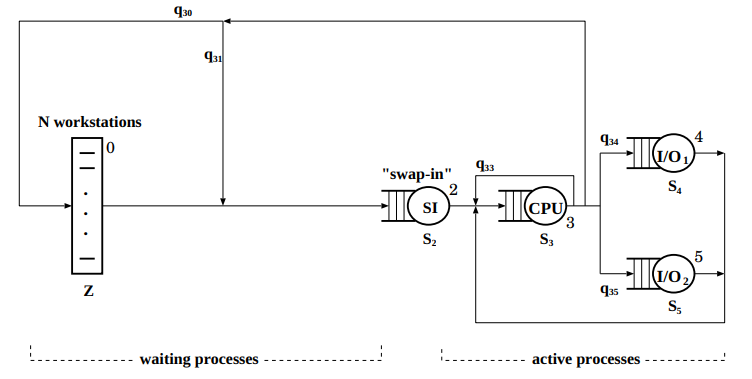
\includegraphics[width=0.8\textwidth]{Images/simplified_model.png}
\\And summarize some data:
\begin{displaymath}
    \begin{aligned}
        S_2 = 210ms  &  & S_3= 2.7ms     &  & S_4 = 40ms    &  & S_5=180ms      \\
        q_{3,0}= 0.4 &  & q_{3,1}=0.6    &  & q_{3,3} = 0.9 &  & q_{3,4}= 0.065 \\
                     &  & q_{3.5}= 0.025 &  & q_{3,6}=0.01  &  &
    \end{aligned}
\end{displaymath}
Based on this data, it becomes evident that the provided approximation is plausible. Given a process with a 0.9 probability of returning with a mean service time of 2.7, and considering our original model where clients exhibit a mean service time of 27 ms and a fixed CPU slice time of 2.7 ms, we anticipate that a customer will be rescheduled in the CPU nearly nine additional times following the initial scheduling. \\

From the previous data we can extract this matrix
\begin{displaymath}
    \begin{bmatrix}
        0     &  & 1     &  & 0   &  & 0     &  & 0     \\
        0     &  & 0     &  & 1   &  & 0     &  & 0     \\
        0.004 &  & 0.006 &  & 0.9 &  & 0.065 &  & 0.025 \\
        0     &  & 0     &  & 1   &  & 0     &  & 0     \\
        0     &  & 0     &  & 1   &  & 0     &  & 0     \\
    \end{bmatrix}
\end{displaymath}

From which we can extract the following system of equations
\begin{displaymath}
    \begin{cases}
        V_0=0.004V_3           \\
        V_2=V_0+0.006V_3       \\
        V_3=V_2+0.9V_3+V_4+V_5 \\
        V_4=0.065V_3           \\
        V_5= 0.025V_3
    \end{cases}
\end{displaymath}
with the additional equation $V_0=1$. Resolving this system lead to the computation
all $V_i$
\begin{displaymath}
    \begin{cases}
        V_0=1     \\
        V_3=250   \\
        V_2=2.5   \\
        V_4=16.25 \\
        V_5=6.25
    \end{cases}
\end{displaymath}

From this computes $V_i$ is possible to detect which of the station is the bottleneck of the system
by considering that $VbS_b= \max_i\{V_iS_i\}$, so let's compute all $V_iS_i$ and find
the greater one.

\begin{displaymath}
    \begin{aligned}
        V_2S_2= 525ms &  & V_3S_3=675ms &  & V_4S_4=650ms &  & V_5S_5= 1125ms
    \end{aligned}
\end{displaymath}
from this calculation we can say that $V_bS_b=V_5S_5=1125ms$ and so , station 5 (IO2) is
our bottleneck. Let's extract some additional information, as the total cycle time when $N=1$ ,i.e Y(1)
\begin{displaymath}
    D=\sum_{i=1}^{N}D_i=\sum_{i=1}^{N}V_iS_i + V_0S_0=7975ms
\end{displaymath}
Thus we can also calculate the saturation point $N^*$ of this system, after which we can expect
the total response time will increase.
\begin{displaymath}
    N^*=\frac{Y(1)}{V_bS_b}=\frac{D}{V_bS_b}=\frac{7975ms}{1125ms}=7.08
\end{displaymath}
\subsection{MVA analysis}
Starting from the previous matrix is possible to compute various measures using the MVA algorithm for Load Indipendent and Delay stations. In order to compute the visits vector is possible to resolve the matrix Q as system of linear equations $V=VQ$, in this case the solution comes by initializing the vector $V = [1,0,0,0,0]$ and then dot multiply it repeatly for the matrix Q. In python this can be done with the following script :\pagebreak
\begin{lstlisting}[language=python]
    matrix = np.array([
    [0,1,0,0,0],
    [0,0,1,0,0],
    [0.004,0.006,0.9,0.065,0.025],
    [0,0,1,0,0],
    [0,0,1,0,0]],np.dtype('d'))

    v = np.zeros(len(matrix))
    v[0] = 1
    for i in range(1000):
        v = v @ matrix
        pass
    for i in range(1,len(v)):
        v[i] = v[i]*(1/v[0])
        pass
    v[0] = 1
    \end{lstlisting}
Applying MVA to those values we obtain the subsequent values.

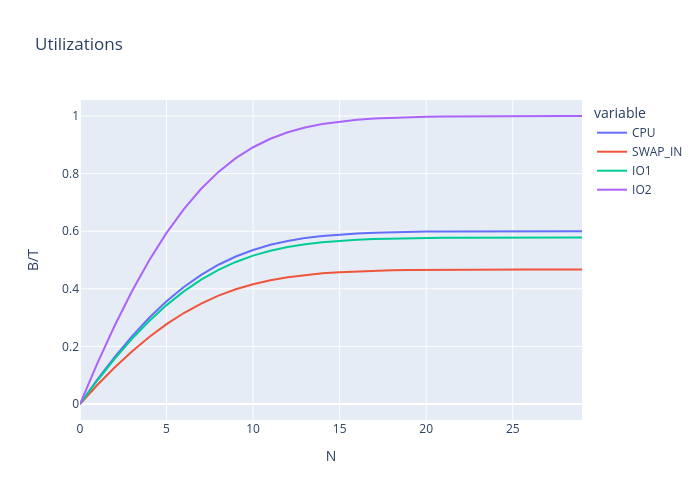
\includegraphics[width=0.9\textwidth]{./Images/Utilizations.png}\\
From the utilization functions we can conclude that the bottleneck station is IO2, as confirmed by the bottleneck analysis. Also becomes evident that after the saturation point ($N \approx7$) the growth of utilization tend to diminish despite the linear increase of N.
\\
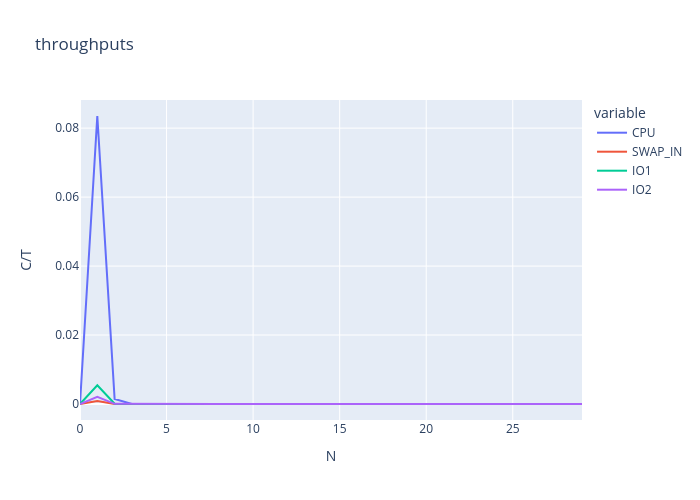
\includegraphics[width=0.9\textwidth]{Images/throughputs.png}
\\
Also from the throughputs the same statement can be reached, but with a particular observation on the CPU, that gradually stop the increasing of the throughput as N becomes larger then 7. This phenomena is similar to a very well known problem in the operative system ecosystem: thrashing. In this case the thrashing is caused by the massive use of the IO2 from the processes involved, so the throughput of the CPU will not decrease but remain steady as it will depend entirely on the process capacity of the IO2.
\\
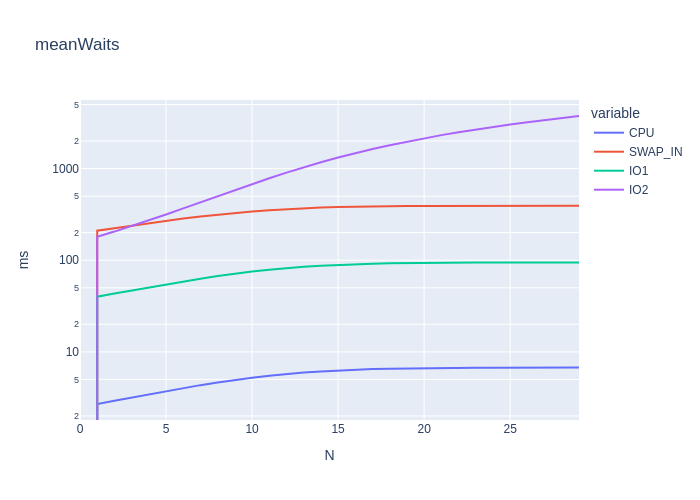
\includegraphics[width=0.9\textwidth]{Images/meanWaits.png}
\\
Mean waits also confirm that the bottleneck station is the IO2, since all other don't increase their mean wait time at the increase of N.
\\
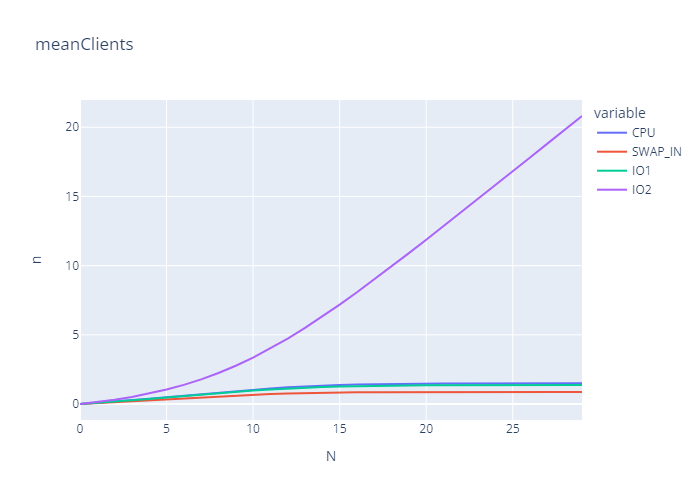
\includegraphics[width=0.9\textwidth]{Images/meanClients.png}
\\
In this graph the tendency of the IO2 station to be a bottleneck is much visible, since the customers tend to increase the queue size of the IO2 at the increase of N.

Considering the subsystem composed by IO1,IO2 and CPU we can estimate then the active time of a client with little effort, resorting to little's formula
$$
    \bar{w}= \frac{\bar{n}}{\lambda}
$$
since all the clients are coming from the swap in, then it's throughput becomes the arrival rate of the formula. The data show that with N=20 a value of 6630 should be expected.

\subsection{Comparison with the data from the simulator}
A special scenario was used to perform a comparison between the data provided by the simulator and the data provide by MVA. This scenario has special parameters. First of all burst times are distributed according to a negative exponential RV with expected value 2.7 ms, the routing probabilities contemplate the possibility of a process to return immediately to the CPU (0.9). The MPD is set to a very high value and also the time slice parameter. Since in this scenario the mean queue value is distributed differently to the other scenarios, where the MPD was limiting the number of process available in the active part of the system, a new regeneration point is adopted. In this regeneration point every time the tagged customer approach the swap out the system must have 0 clients at the CPU, 0 at the IO1 and 16 at the IO2.

\includegraphics[width=0.9\textwidth]{./Images/meanActiveTime_Simplified_N20.png}

\begin{table}[!ht]
    \centering
    \begin{tabular}{|l|l|l|l|l|l|l|l|}
    \hline
        Station & Measure & R & LB & HB & Samples & Precision & Expected \\ \hline
        CPU & meanclients & 1.48174 & 1.45508 & 1.5084 & 79 & 0.01799 & 1.47487 \\ \hline
        CPU & meanwaits & 6.66375 & 6.5834 & 6.74411 & 79 & 0.01206 & 6.65303 \\ \hline
        IO1 & meanclients & 1.33464 & 1.30503 & 1.36425 & 79 & 0.02219 & 1.34865 \\ \hline
        IO1 & meanwaits & 92.66997 & 91.18805 & 94.15188 & 79 & 0.01599 & 93.59424 \\ \hline
        IO2 & meanclients & 11.87094 & 11.75226 & 11.98962 & 79 & 0.01 & 11.87475 \\ \hline
        IO2 & meanwaits & 2139.17766 & 2112.67305 & 2165.68226 & 79 & 0.01239 & 2142.63856 \\ \hline
        SWAP\_IN & meanclients & 0.86383 & 0.84567 & 0.88198 & 79 & 0.02102 & 0.86804 \\ \hline
        SWAP\_IN & meanwaits & 387.61848 & 381.57996 & 393.65699 & 79 & 0.01558 & 391.56501 \\ \hline
        ActiveTime & cycleTime & 6323.25794 & 6009.10935 & 6637.40653 & 79 & 0.04968 & 6630.26191 \\ \hline
    \end{tabular}
\end{table}


After 20 simulations, as expected, there are times in which the expected value is within the confidence interval and others not. 
\begin{verbatim}
    StationCPU Measure meanwaits HitPercentage 90.0
    StationCPU Measure meanclients HitPercentage 95.0
    StationIO1 Measure meanwaits HitPercentage 90.0
    StationIO1 Measure meanclients HitPercentage 90.0
    StationIO2 Measure meanwaits HitPercentage 95.0
    StationIO2 Measure meanclients HitPercentage 100.0
    StationSWAP_IN Measure meanwaits HitPercentage 95.0
    StationSWAP_IN Measure meanclients HitPercentage 95.0
    Activetimes HitPercentage 90.0%
\end{verbatim}

The expected value of active times, that are the focus of this simulation, were in the confidence interval 90\% of the simulations. Since the expectations are that the expected value is in the confidence interval for $N(1-\alpha)$ times or equivalently $\frac{hits}{N}*100=1-\alpha$, where hits is the number of times the expected value is in the confidence interval, the simulator can be considered a good approximation of the given model.



\section{Second validation step}
In the second validation step a different kind of effort is required, build and extract information from a Markov chain.
\subsection{States definition}
The first step is define how a state is represented. The simplest way is to consider as state a tuple of clients, each element will represent the client that are currently enqueued to each station (N\_Delay, N\_CPU, N\_IO1,N\_IO2), the swap in station is not present because it have service time 0, and so clients are processed instantaneously. 
\begin{lstlisting}[language=python]
class State:
    def __init__(self,Ndelay, Ncpu, Nio1, Nio2,cpuStage = 0) -> None:
        self.Ndelay = Ndelay
        self.Ncpu = Ncpu
        self.cpuStage = cpuStage
        self.Nio1 = Nio1
        self.Nio2 = Nio2
        self.state= [Ndelay,Ncpu,Nio1,Nio2,cpuStage]
        self.descriptor =["Ndelay","Ncpu","Nio1","Nio2","cpuStage"]
        pass
\end{lstlisting}

In this model a state is valid only if the sum of clients in each station is equal to N (the number of workstation that are present in the system). Another condition is that if there is almost 1 client in CPU, the state must be either 1 or 2.

\begin{lstlisting}[language=python,breaklines]
    def isValid(self)->bool:
        if self.Ncpu > 0:
            return (self.cpuStage == 1 or self.cpuStage == 2) and (self.Ncpu + self.Nio1 + self.Nio2 + self.Ndelay) == SystemParameters.numClients
        else:
            return (self.Ncpu + self.Nio1 + self.Nio2 + self.Ndelay) == SystemParameters.numClients
\end{lstlisting}

With this simple statements is possible to define a generator of states by iterating through all the possibilities 

\begin{lstlisting}[language=python,breaklines]
def stage_enumerator(stage: int) -> list[State]:
    Ndelay = 0
    Ncpu = 1
    Nio1 = 2
    Nio2 = 3
    cpuStage = stage
    stages = [0,0,0,0]
    result = []
    while stages[Ndelay] <= SystemParameters.numClients:
        for i in reversed(range(4)):
            stages[i] += 1
            if stages[i] <= SystemParameters.numClients: break
            elif i > 0 : stages[i] = 0
            pass
        state= State(stages[Ndelay], stages[Ncpu], stages[Nio1],stages[Nio2],stage)
        if state.isValid(): result.append(state)
        pass
    return result
\end{lstlisting}

The result will be all the valid nodes for the graph, the next step is to correctly define all the possible transition in the system.

\subsection{Transition definition}
A transition is an edge in the graph, it represent the probability that the chain move from a given state to an adjacent state. A transition can be only:
\begin{itemize}
    \item A client pass from CPU to IO1 
    \item A client pass from CPU to IO2 
    \item A client pass from IO2 to CPU
    \item A client pass from IO1 to CPU
    \item A client pass from DELAY to CPU
    \item A client pass from CPU to DELAY
\end{itemize}

\begin{lstlisting}[language=python]
class Transition:   
    class TransitionType:
       UNKNOWN = -1
       CPU_TO_IO1 = 1
       CPU_TO_IO2 = 2
       IO2_TO_CPU = 4
       IO1_TO_CPU = 5
       DELAY_TO_CPU = 6
       CPU_TO_DELAY = 7
       pass

def __init__(self, head: State, tail : State) -> None:
       self.head = head
       self.tail = tail
       self.type = Transition.TransitionType.UNKNOWN
       self.detectType()
    pass
\end{lstlisting}

Not all possible edges in the graph are valid, so it is necessary to impose some constraints accepted ones. Since the chain is a directed graph let's give some definitions, the head of an edge is the actual state considered, the tail is the destination of the transition. Fixed those elements a transition is valid only if:
\begin{itemize}
    \item The tail has one station with less one client than the head 
    \item The tail has one station with more one client than the head 
\end{itemize}
in this manner only the node that are one step away are considered. 

\begin{lstlisting}[language=python,breaklines]
def transitionIsValid(self):
    #check cpu stage
    if self.head.cpuStage != self.tail.cpuStage:
       if self.head.Ncpu < self.tail.Ncpu and self.tail.Ncpu > 0 and self.head.Ncpu > 0: return False
       pass
    changed = 0
    def validate_var(a , b):
       nonlocal changed 
       if abs(a - b) > 1 : return False 
       if abs(a-b) == 1 and changed > 1: return False
       if abs(a-b) == 0 : return True
       else: changed += 1         
       return True
    for i in range(len(self.head)):
       if not validate_var(self.head[i],self.tail[i]): return False
       pass
    return True
\end{lstlisting}

At this point is possible to define the type of the transition simply by observing what station decremented its customer and the one that increased. A transition will be than of type: 

\begin{itemize}
    \item a transition from CPU to IO if a decrement from CPU and an increment to IO is observed and vice versa a transition from IO to CPU 
    \item a transition from CPU to Delay if a decrement from CPU is observed and an increase to Delay is observed, vice versa a transition from Delay to CPU.
\end{itemize}

\begin{lstlisting}[language=python]
    def detectType(self):
    #return so that the value remains unknown
    if not self.transitionIsValid() : return
    (decrement,increment)= self.detectMovement()
    if decrement == "ERROR" or increment == "ERROR" : return 
    elif decrement == "Ncpu" and increment == "Nio1": self.type = Transition.TransitionType.CPU_TO_IO1
    elif decrement == "Ncpu" and increment == "Nio2" : self.type = Transition.TransitionType.CPU_TO_IO2
    elif decrement == "Nio1" and increment == "Ncpu" : self.type = Transition.TransitionType.IO1_TO_CPU
    elif decrement == "Nio2" and increment == "Ncpu" : self.type = Transition.TransitionType.IO2_TO_CPU
    elif decrement == "Ndelay" and increment == "Ncpu" : self.type = Transition.TransitionType.DELAY_TO_CPU
    elif decrement == "Ncpu" and increment == "Ndelay" : self.type = Transition.TransitionType.CPU_TO_DELAY
    pass
\end{lstlisting}

So now for all transition types is possible to define a transition probability. \pagebreak

\subsubsection{CPU Transition}

The CPU possible transition must take in consideration the current state (1 or 2) of the client in process. Starting from the departures let's define a simple, yet useful function L (leave) that assume values 
$$L(h,t)=
\begin{cases}
    \frac{1}{u_1}*\alpha &  H_1 \rightarrow T_1 \\
    \frac{1}{u_2}*\alpha & H_2 \rightarrow T_1\\
    \frac{1}{u_1}*\beta & H_1 \rightarrow T_2 \\
    \frac{1}{u_2}*\beta & H_2 \rightarrow T_2\\
    \frac{1}{u_1} & H_1 \rightarrow T_0\\
    \frac{1}{u_2} & H_2 \rightarrow T_0
\end{cases}
$$
Where $u_1,u_2,\alpha,\beta$ are the constants that describe the hyper exponential of the cpu. $h$ and $t$ are the head and the tail of the transition: $H_1$ means that the head is in stage 1,same for $H_2$ with stage 2 and the tail that is T. Special case is $T_0$ that means the tail has no client in the cpu, so alpha and beta are not considered.  

\begin{lstlisting}[language=python]
def CpuL(self):
    l = 1/SystemParameters.u1 if self.head.cpuStage == 1 else 1/SystemParameters.u2
    if self.tail.Ncpu > 0:
       l *=  SystemParameters.alpha if self.tail.cpuStage == 1 else SystemParameters.beta
       pass
    return l
\end{lstlisting}

The next steps involve to consider where the client is directed when leaving, destinations can be: Delay and IOs, also CPU to CPU are valid transitions, but useless because the values obtained from this transition will be deleted when the chain will be "normalized". So the probability will be $p=L(h,t)*q_{3,4/5}$ if the client is directed towards the IOs and $p=L(h,t)*q_{3,0}$ if the client is directed to the delay station. 

\begin{lstlisting}[language=python]
 def CpuToIo(self):      
    return self.CpuL()*SystemParameters.qio1 if self.type == Transition.TransitionType.CPU_TO_IO1 else self.CpuL()*SystemParameters.qio2
 
 def CpuToDelay(self):
    return self.CpuL()*SystemParameters.qoutd
\end{lstlisting}

Let's now consider all the transition that goes to the CPU i.e. arrivals. Since the service time of the swap in is 0, is possible to assume that an arrival can come from the delay station directly or from the IOs. 
\section{Simulator description}
\subsection{Brief description of the implementation}
The simulator is substantially a shell. The program loads at the beginning the skeleton of the simulator composed by an OS object. Such object hold the description of the model composed by a Round Robin station (class CPU), a delay station (class DelayStation) and all the other First Come First Served (class FCFSStation). The OS Object inherit from scheduler that hold the main event queue and manage all the operations inside the simulator. OS also inherit from the class Simulator, that substantially contains all the functions that are need to pilot the execution, such as dequeue an event , route it to the right station and so on. The environment of simulation is divided in 3 abstraction layers:
\begin{itemize}
    \item class SimulationEnvironment
    \item class SimulationResult
    \item class SimulationShell
\end{itemize}
\subsubsection{SimulationEnvironment}
This class hold the setup functions for the base system and each scenario. Scenarios are a short way to describe the regeneration point for that scenario and the parameter for the simulation (for example the cpu slice time). In all the four case described the regeneration point is the same, but the parameter (especially for the CPU) are different. This class also contains the SimulationResult data strucuture, which holds all the accumulators.
\subsubsection{SimulationResult}
SimulationResult class hold all the accumulator used to display the result of the simulator, it contains various function for register 2 particular measure of all the station involved: mean waits and mean clients. At the end of each regeneration cycle the measure are extracted from the OS class.
\subsubsection{SimulationShell}
this class hold all the functions need to make the program interactive, in the section Available commands various input can be used to manipulate the simulator. The principal facilities of this class let the user to create a Command structure, which pair a sequence of character to an action.
\subsection{Available commands}
\begin{itemize}
    \item help: display an help with all the commands
    \item verbosity <list|sourceName> [int] : let the user to select a verbosity for a source, the sources can be listed with list. Note that all the station have verbosity 1 in order to not display the actual processing of the events.
    \item start: manually start the simulator
    \item stop: manually stop the simulator
    \item init: initialize the system , it is needed after each call to scenario.
    \item clock: display the actual clock of the simulation.
    \item ne [int]: process a certain number of events
    \item seed: set the seed for the simulator
    \item hreset: reset completely the state of the simulator
    \item exit: quit the program
    \item regstats: display the statistics on hit and call of regeneration point , each hit correspond to an event that call the regeneration point, each call correspond to the regeneration point being satisfied.
    \item env: Display the environment variables (SystemParameters) that describe the scenario used for the simulator (MPD, slice ecc\dots)
    \item lstats: Display the actual status of the stations , B=busy time, O= observation time, A=arrivals,C=completions,N: sysclients, W:meanWaits (sample mean), MAXN: max sysclients observed, AN: area of N (sysclients*interval), AS:area of S ((sysclients-1)*interval).
    \item lqueue <name>: Display the actual status of all the queues
    \item scenario <list|scenarioname>: set the scenario for the simulation. A brief description of the available scenario is available in the section Scenarios.
    \item nr <numCycles:0+|untilPrecisionReached:-1> <showMeasure:1|0>: compute the n regeneration cycle or stop when the requested precision (0.05) is reached (using -1 as argument). The second argument ask to display or not the measure after each regeneration cycle (0 false, 1 true).
    \item na <CPU|IO1|IO2|SWAP\_IN>: Execute the simulation until an arrival is detected to the station listed.
    \item nd <CPU|IO1|IO2|SWAP\_IN>: Execute the simulation until a departure is detected to the station listed.
    \item nn <seed:int> <numSimulations:int> <showMeasure:1|0> : Execute a fixed number of simulation reaching the precision requested every time, at the end of each simulation it will compare with MVA result and tell if the confidence interval has the true mean or not.
    \item ltgtstats: print the cycle time catch by the tagged customer
    \item lmeasures: print all the collected measure
    \item reset\_measures: manually reset all the accumulators

\end{itemize}
\end{document}